\chapter{最小生成树其他算法}

\begin{introduction}
	\item red/blue算法
	\item Boruvka算法
\end{introduction}

本章将介绍求解最小生成树的red/blue算法和Boruvka算法。

\section{red/blue算法}

\subsection{基本概念}
下面给出red/blue算法有关内容的定义
\begin{definition}{割(cut)}{cut}
	S$\in$V,S$\neq \emptyset$,点集V被划分成互补的子集S和V/S。
\end{definition}

\begin{definition}{割边集(cutset)}{cutset}
    对于图G的顶点集V的割X、Y,图G的边集E中连接两集合X、Y的所有边的集合叫做这个割的割边集(cutset)。
\end{definition}

\begin{definition}{Red Rule}{Red Rule}
    找到图G中不含红色边的环C,从C中未被染色的边中选出边权最大的边将其染成红色。
\end{definition}

\begin{definition}{Blue Rule}{Blue Rule}
    找到图G中不含蓝色边的割边集D,从D中未被染色的边中选出边权最小的边将其染成蓝色。
\end{definition}

\subsection{算法运行步骤}
1. 初始化:对于给定的图G,将所有边标记为未染色。

2. 在图G中同时运行Red Rule和Blue Rule (可并行运行),直到所有边均被染色为止。

3. 图G中所有的蓝色边即为图G的最小生成树。

算法具体执行过程如\autoref{fig:redblue}
\begin{figure}[hbt]
	\centering
	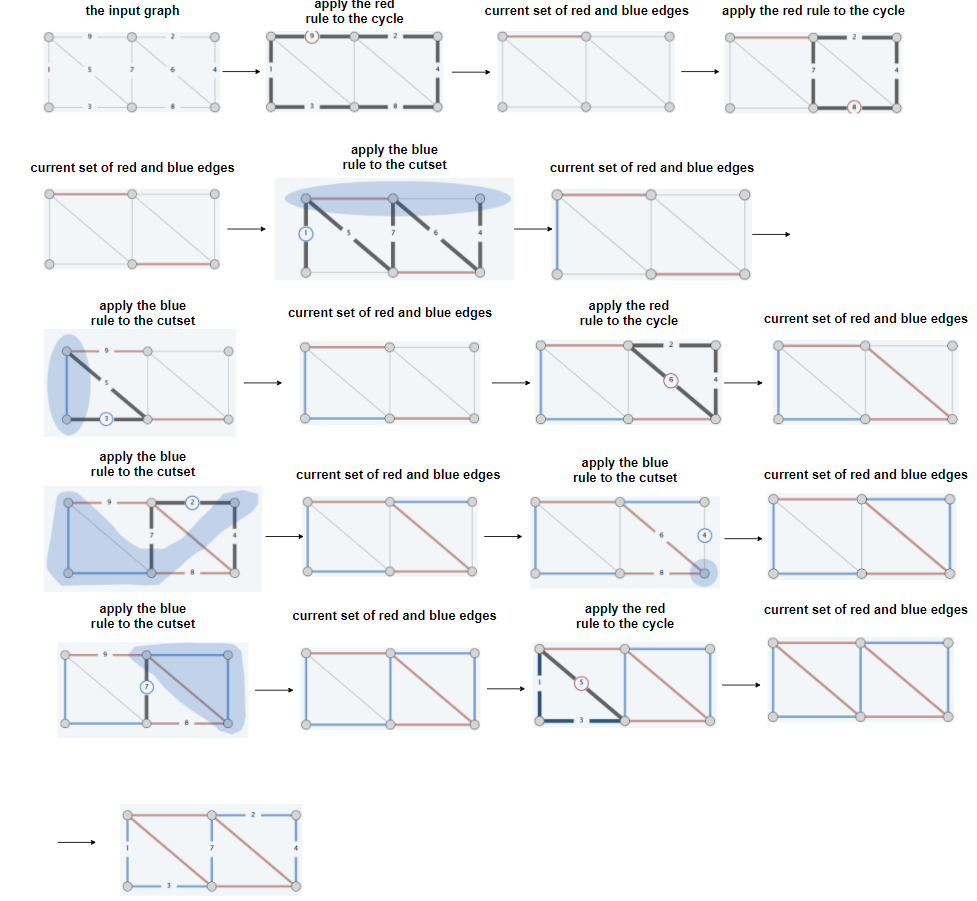
\includegraphics[scale=0.4]{image/redblue.png}
  \caption{red/blue算法执行过程图解}\label{fig:redblue}
\end{figure}

\subsection{算法正确性证明}\label{sec:redblue-proof}
\noindent(1)最优性:Blue Rule染色所得边为最小边

对于图G中的一个割边集D及D中边权最小的边minEdge,如果在Blue Rule运行过程中被染色的是割边集D的其他边biggerEdge,
则可以在最后得到的MST中将biggerEdge从中删除然后将minEdge加入到MST中,可以得到更小的最小生成树。产生矛盾。所以Blue Rule染色所得边为最小边。

\noindent(2)合法性:算法所得所有蓝边为无环连通图

由于Blue Rule可知每次选边都不会成环。下证所得为连通图,假设最后所得所有蓝边构成的图不连通或仍然有点未被蓝边连接。

对于第一种情况,则任选某一蓝边的一个顶点并从该顶点开始的所有能通过蓝边的顶点记为集合X,
S与V/S构成图G的一个割,由Red Rule中所选环C不含红色边可知其割边集不可能全部被染成红色,则说明一定有未染色的边,再应用一次Blue Rule即可增大S的点的个数,
重复上述过程直到S=E;对于第二种情况,由于孤立点必不可能在某个环中,所以连接该点的边一定不会被Red Rule染成红色,所以此时应用一次Blue Rule即可使得该点被蓝边连接。综上,算法所得所有蓝边为连通图

\section{Boruvka算法}
\subsection{算法运行步骤}
1. 初始化:对于给定的图G,将所有边标记为未染色;将每个顶点作为一个连通块。

2. 对于所有蓝边连成的连通块应用Blue Rule并将所有Blue Rule选中的边染成蓝色,直到只有一个连通块。

3. 最后得到的蓝边连成的连通块即为图G的最小生成树。

算法具体执行过程如\autoref{fig:boruvka}
\begin{figure}[h]
	\centering
	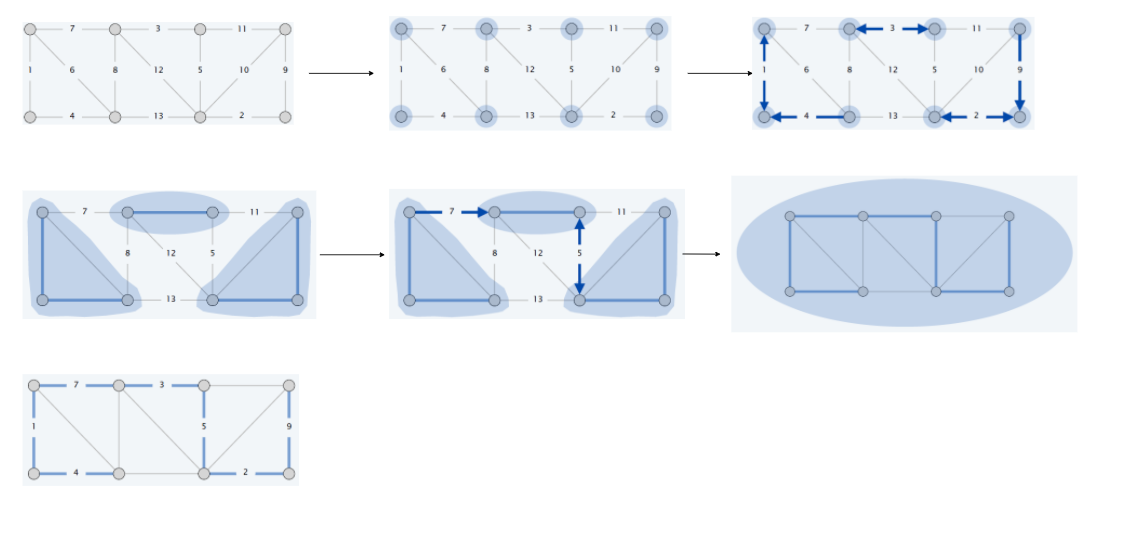
\includegraphics[scale=0.4]{image/boruvka.png}
  \caption{boruvka算法执行过程图解}\label{fig:boruvka}
\end{figure}

算法复杂度分析:每次应用Blue Rule后连通块数量至少减半,每次都要遍历所有边,所以算法串行时间复杂度为O(E$\log V$),并行时间复杂度为O(E)。

\subsection{算法正确性证明}
\noindent(1)最优性:根据~\ref{sec:redblue-proof}中的证明:Blue Rule染色所得边为最小边。

\noindent(2)合法性:一定不会构成环。如果存在环说明一个点的最小连边有两个,与Blue Rule矛盾。
